\documentclass[10pt]{beamer}

\mode<presentation>
{
  \usetheme[height=1.25cm]{Madrid}
  \setbeamertemplate{navigation symbols}{}
  \setbeamercolor{alerted text}{fg=illini}
}

\graphicspath{{figs/}}

\usebackgroundtemplate{
\includegraphics[width=\paperwidth,height=\paperheight]{uc-background}}

\usepackage[english]{babel}
\usepackage{epsfig,subfigure,bm}
\usepackage{multimedia}
\usepackage{psfrag}
\usepackage{animate}

% \usefonttheme{metropolis} % default family is serif
%%%%%% Begin of my macros and options

\setbeamertemplate{section in toc shaded}[default][55]
\setbeamertemplate{subsection in toc shaded}[default][55]
\setbeamercolor{block title}{fg=white,bg=illini}
\setbeamercolor{block body}{fg=black,bg=mygrey}

\setbeamercolor{emphprimary}{fg=CBlue}
\setbeamercolor{emphsecondary}{fg=illini}
\setbeamercolor{emphtertiary}{fg=mygreen}
\definecolor{darkForestGreen}{rgb}{.1,1,.1}
\definecolor{veryLightGray}{rgb}{.9,.9,.9}
\definecolor{greenApple}{rgb}{.3,.9,.3}

\setbeamercolor{frametitle}{bg=CBlue}   
\setbeamercolor{title}{bg=CBlue}

\usepackage{amsmath,amssymb,amsxtra,amsthm}
\usepackage{algorithm,algorithmic}
\usepackage{natbib}
\usepackage{bibentry}
\usepackage{xspace}
\usepackage{changepage}

\definecolor{myblue}{rgb}{.2,.2,.7}
\definecolor{myred}{rgb}{.7,.2,.2}
\definecolor{mygreen}{rgb}{.2,.7,.2}
\definecolor{mygrey}{rgb}{0.9,0.9,0.9}
\definecolor{CBlue}{cmyk}{1,0.25,0,0}
\definecolor{illini}{rgb}{0.98,0.4,0.05}
\definecolor{black}{cmyk}{0,0,0,1}

\newcommand{\myemph}[1]{{\usebeamercolor[fg]{emphprimary}
    \textbf{#1}}}
\newcommand{\myemphalt}[1]{{\usebeamercolor[fg]{emphsecondary}
    \textbf{#1}}}

\graphicspath{{figs/}}

\title[Math for Robotics] % (optional, use only with long paper titles)
{CSE276C - Calculus of Variation}

\author[H.~I. Christensen] % (optional, use only with lots of authors)
{Henrik I.~Christensen}
% - Give the names in the same order as the appear in the paper.  -
% Use the \inst{?} command only if the authors have different
% affiliation.

\AtBeginSection[]
{
   \begin{frame}
       \frametitle{Outline}
       \tableofcontents[currentsection]
   \end{frame}
}

\institute[UCSD] % (optional, but mostly needed)
{
  \begin{minipage}[c]{.2\textwidth}
    
\includegraphics[width=.65\linewidth]{ucsealnew}%
  \end{minipage}%
  \begin{minipage}[c]{.6\textwidth}
    \small
%%    \begin{center}
      Computer Science and Engineering\\
      University of California, San Diego\\
      \myemph{\url{http://cri.ucsd.edu}}\\          
%%    \end{center}

  \end{minipage}
%%  \vspace*{1ex}
}
%% - Use the \inst command only if there are several affiliations.
%% - Keep it simple, no one is interested in your street address.

\bigskip

\date[Nov 2020]% (optional, should be abbreviation of conference name)
{\small%
  November 2020}

\begin{document}
  
\nobibliography{/Users/hic/Dropbox/bibliography/bib-file}
\bibliographystyle{plain}

\begin{frame}[plain]
  \titlepage
\end{frame}


\begin{frame}
  \frametitle{Introduction}
  \begin{itemize}
  \item Going a bit more abstract today. 
  \item Calc of variations is tightly coupled to mechanics
  \item We will only covers the very basics 
  \item Entire courses at UCSD - MATH201C
  \end{itemize}
\end{frame}


\begin{frame}
  \frametitle{Applications}
  \begin{itemize}
  \item Path Optimization
  \item Vibrating membranes
  \item Electrostatics
  \item Machine vision - reconstruction
  \item VIsion - image flow, ...    
  \end{itemize}
\end{frame}

\begin{frame}
  \frametitle{Introduction (cont)}
  \begin{itemize}
  \item We have see the principle
    \begin{itemize}
    \item To minimize P is to solve P' = 0
    \end{itemize}
  \item So far we have looked at finite dimensional problems
    \begin{itemize}
    \item f: $\mathcal{R}^n \rightarrow \mathcal{R}$
    \end{itemize}
    Looking at N numbers to minimize f
  \item In infinite dimensional problems we are considering an continuum
  \item What about functionals - (functions of functions)? 
  \end{itemize}
\end{frame}

\begin{frame}
  \frametitle{Example}
  \begin{itemize}
  \item Suppose we connect two points in the plane $(x_0, y_0)$ and
    $(x_1, y_1)$ by a curve of the form y = y(x).
    \centerline{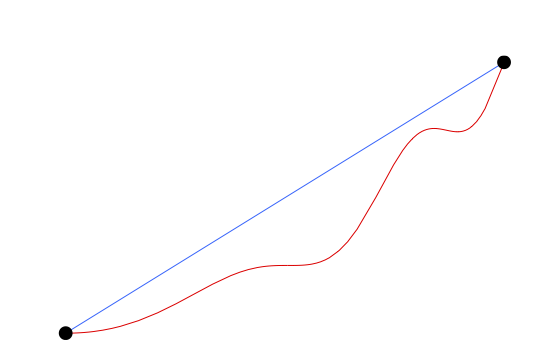
\includegraphics[height=4cm]{basic-curve}}
  \item The length if the curve can be written
    \[ L(y) = \int_{x_0}^{x_1} \sqrt{1 + (y')^2} dx \]
    L is a functional. 
  \item Find the shortest curve between the two points. 
  \end{itemize}
\end{frame}

\begin{frame}
  \frametitle{Similar problems}
  \begin{itemize}
  \item Shortest path connecting a non-planar curve, say sphere
  \item Minimal surface of revolution generated by a connected curve
  \item Shortest curve with a given area below it
  \item Closed curve of a given perimeter that encloses the largest area
  \item Shape of a string hanging from two points under gravity
  \item Path of light travelling through an inhomogenous curve
  \end{itemize}
\end{frame}


\begin{frame}
  \frametitle{Euler's Equation}
  \begin{itemize}
  \item The principle of 
    \begin{itemize}
    \item To minimize P is to solve P' = 0
    \end{itemize}
  \item Rather than solving the integral it is an advantage to
    consider the differential equation. 
  \item The differential equation is called Euler Equation. 
  \item We will derive it shortly
  \end{itemize}
\end{frame}


\begin{frame}
  \frametitle{Consider for a minute}
  \begin{itemize}
  \item Suppose $ f: \mathcal{R}^n \rightarrow \mathcal{R}$ what does it mean for $x^*$ to be a local extremum of f? 
    \begin{enumerate}
    \item We must have $f(x) \geq f(x^*)$ for every x in some neighborhood
    \item A necessary condition $\nabla f(x^*) = 0$ i.e., that $\frac{\partial f}{\partial x_i} = 0$ for all i. 
    \end{enumerate}
  \item For P the equivalent would be say
    \begin{enumerate}
    \item $P: C^2(\mathcal{R}^n) \rightarrow \mathcal{R}$ and
    \item $f \rightarrow P(f)$
    \end{enumerate}
  \item what does it mean for $f^*$ to be an extremum of P?
  \end{itemize}
\end{frame}

\begin{frame}
  \frametitle{Optimal functional? }
  \begin{itemize}
  \item What would be conditional for a functional?
    \begin{enumerate}
    \item We need $P(f) \geq P(f^*)$ for every functional close to $f^*$
      \begin{itemize}
      \item So what is a neighborhood of a function?
      \end{itemize}
    \item Need a generalized gradient
      \[
        P( f^* + \delta f ) \approx P(f^*)
      \]
    \end{enumerate}
  \item Still very hand wavy
  \end{itemize}
\end{frame}

\begin{frame}
  \frametitle{Simplest problem}
  \begin{itemize}
  \item Lets start with a simple problem
  \item Minimize $J(y) = \int_{x_0}^{x_1} F(x, y, y') dx$ with $y, F in C^2$
  \item Suppose $y^*$ minimizes J it would then be true
    \begin{enumerate}
    \item In a neighborhood of $y^*$ then $J(y) \geq J(y^*)$
    \item $\delta J = 0$ for a variation $\delta y$ is
      \[
        \delta J(y^*) = J(y^* + \delta y) - J(y^*)
      \]
    \end{enumerate}
  \item What are the necessary conditions for this to be valid
  \end{itemize}
\end{frame}

\begin{frame}
  \frametitle{Neighborhood Evaluation}
  \begin{itemize}
  \item Lets start by showing optimality in a neighborhood
  \item Let $y \in C^2[x_0, x_1]$ such that $y(x_0) = y(x_1) = 0$
  \item Let   $\epsilon \in \mathcal{R}$ be a value
  \item Lets consider a one-parameter family of functions
    \[
      y(x) = y^*(x) + \epsilon y(x)
    \]
  \item Where $y^*$ is the (unknown) optimal function
  \item Define $\Phi: \mathcal{R} \rightarrow \mathcal{R}$ by
    \[
      \Phi(\epsilon) = \int_{x_0}^{x_1} F(x, y, y') dx
    \]
  \item If $|\epsilon|$ is small enough then all variants of
    $y^* + \epsilon y$ lie in a small neighborhood of $y^*$,
    therefore $\Phi$ attains a local minimum at $\epsilon = 0$
  \item Thus it must be true that  $\Phi'(0) = 0$
  \end{itemize}
\end{frame}

\begin{frame}
  \frametitle{So what is $\Phi{'}$?}
  \begin{itemize}
  \item We know that
    \[
      \Phi(\epsilon) = \int_{x_0}^{x_1} F(x, y, y{'}) dx
    \]
  \item So it must be true that
    \[
      \Phi'(\epsilon) = \frac{d}{d \epsilon} \int_{x_0}^{x_1} F(x, y, y{'}) dx
    \]
  \item Given that we have a $C^{2}$ domain we can reverse the order of
    integration and differentiation, so that
    \[
      \Phi{'}(\epsilon) =  \int_{x_0}^{x_1} \frac{d}{d \epsilon} F(x, y, y{'}) dx
    \] \pause or
    \[
      \Phi{'}( \epsilon ) =  \int_{x_0}^{x_1} \left(
        \frac{\partial}{\partial y} F(x, y^{*} +  \epsilon y, y^{*'}+ \epsilon y{'} ) y +  
        \frac{\partial}{\partial y{'}} F ( x, y^{*} + \epsilon y, y^{*'}+ \epsilon y{'} ) y{'} 
        \right) dx
    \]
  \item We know that
    \[
      \Phi{'}(0) = 0 = \int_{x_0}^{x_1} \left( 
       \frac{\partial}{\partial y}  F ( x, y^{*}, y^{*'} ) y + 
       \frac{\partial }{\partial y{'}}  F( x, y^{*} , y^{*'} ) y{'} 
       \right)  dx
    \]
  \end{itemize}
\end{frame}

\begin{frame}
  \frametitle{Still more $\Phi{'}$}
  \begin{itemize}
  \item We can write this more compactly
    \[
      \Phi{'}(0)= \int_{x_0}^{x_1} \left( F_y y + F_{y'} y' \right) dx
    \]
  \item Using integration by parts we get
    \[
      \begin{array}{rcl}
        \int_{x_0}^{x_1} F_{y'} y' dx &=& \left. F_{y'} y \right\vert_{x_0}^{x_1} - \int_{x_0}^{x_1} y \frac{d}{dx} F_{y'} dx\\
        &=& - \int_{x_0}^{x_1} y \frac{d}{dx} F_{y'} dx\\
      \end{array}
    \] with this we can rewrite
    \[
      \Phi{'}(0)= \int_{x_0}^{x_1} \left[ F_y - \frac{d}{dx} F_{y'} \right] y dx = 0
    \] as this has to apply for any function y it must be true that
    \[
      F_y - \frac{d}{dx} F_{y'} = 0 \mbox{ on } [x_0, x_1]
    \]
  \item This is called Euler's Equation
  \end{itemize}
\end{frame}

\begin{frame}
  \frametitle{Side comment}
  \begin{itemize}
  \item The Euler Equation is essentially a ``directional derivative''
    in the direction of y
  \item Going back to earlier - $\delta J$ is finding a function $y^*$
    where J is stationary. 
  \item We are only considering the basics here. 
  \end{itemize}
\end{frame}

\begin{frame}
  \frametitle{Shortest path problem}
  \begin{itemize}
  \item Remember the initial question of shortest path? 
  \item Recall:
    \[
      L(y) = \int_{x_0}^{x_1} \sqrt{1 + y'^2} dx
    \] with $y_0 = y(x_0)$ and $y_1 = y(x_1)$
  \item So $F(x, y, y') = \sqrt{1 + y'^2}$
    \[
      F_y = 0 \mbox{~~~~~~ and ~~~~~} F_{y'} = \frac{y'}{\sqrt{1+y'^2}}
    \]    
  \item Euler Equations reduces to
    \[
      \frac{d}{dx} \frac{y'}{ \sqrt{1+y'^2} } = 0
    \]
  \end{itemize}
\end{frame}

\begin{frame}
  \frametitle{The shortest path?}
  \begin{itemize}
  \item So 
    \[
      \frac{ y' }{ \sqrt{1+y'^2} } = c
    \]
  \item we can rewrite
    \[
      \begin{array}{rcl}
        y'^2& = & c^2 (1+y'^2)\\ 
        y'  & = & \pm \frac{c}{\sqrt{1-c^2}} = m \mbox{ ~~ just a constant} \\ 
        y'  & = & m\\ 
        y   & = & mx + b \\ 
      \end{array}
    \]
    surprise it is the equation for a straight line!
    
  \end{itemize}
\end{frame}

\begin{frame}
  \frametitle{How about contrained optimization?}
  \begin{itemize}
  \item Supposed we are supposed to find shortest curve with a fixed area below?
    \centerline{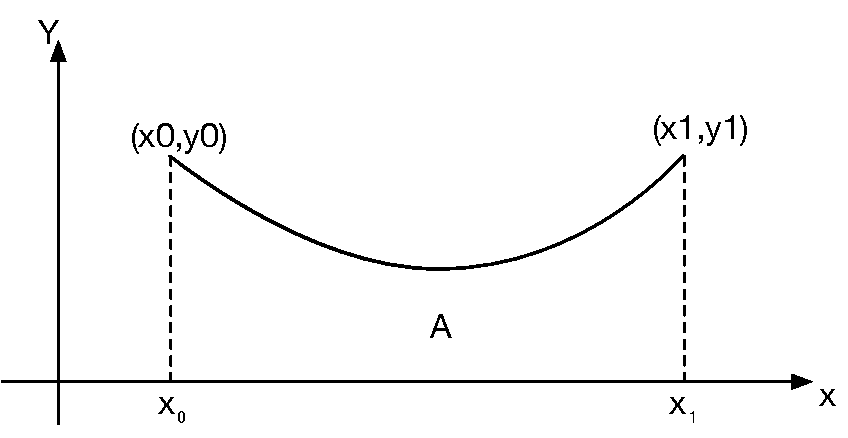
\includegraphics[height=5cm]{constrained}}
  \item The area is given to be A and we have end-points? 
  \end{itemize}
\end{frame}

\begin{frame}
  \frametitle{Constrained optimization}
  \begin{itemize}
  \item Our objective is then to optimize
    \[
      \begin{array}{rcl}
        L(y) &=& \int_{x_0}^{x_1} \sqrt{ 1 + y'^2} dx\\[3mm]
        A    &=& \int_{x_0}^{x_1} y dx\\
      \end{array}
    \]
  \item where the second term is our constraint
  \item An instance of a general class of problems called isoperimetric problems
  \end{itemize}
\end{frame}

\begin{frame}
  \frametitle{Isoperimetric problems}
  \begin{itemize}
  \item The simplified formulation is\\
    
    \begin{tabular}{ll}
      Minimize & $J(y) = \int_{x_0}^{x_1} F(x,y,y') dx$\\
      Subject to & $K(y) = c$ \\
      where & $K(y) = \int_{x_0}^{x_1} G(x, y,y') dx$
    \end{tabular}
  \end{itemize}
\end{frame}

\begin{frame}
  \frametitle{Constrained Optimization (cont.)}
  \begin{itemize}
  \item We can use a combination of variational techniques and Lagrange multipliers to solve such problems
  \item We can define two functions
    \[
      \begin{array}{rcl}
        \Phi(\epsilon_1,\epsilon_2) & = & \int_{x_0}^{x_1} F(x, y^{*} + \epsilon_1 y + \epsilon_2 \xi, y^{*'} + \epsilon_1 y' + \epsilon_2 \xi {'}) dx\\
        \Psi(\epsilon_1,\epsilon_2) & = & \int_{x_0}^{x_1} G(x, y^{*} + \epsilon_1 y + \epsilon_2 \xi, y^{*'} + \epsilon_1 y' + \epsilon_2 \xi {'}) dx\\
      \end{array}
    \]
  \item Here $y^*$ is the unknown function and $y \mbox{ and } \xi$
    are two $C^2$ functions that vanish at the end-points
  \item So we want to minimize $\Phi$ subject to the constraint
    $\Psi$. We know there is a local minimum at
    $\epsilon_1 = \epsilon_2 = 0$
  \end{itemize}
\end{frame}

\begin{frame}
  \frametitle{Constrained Optimization (Cont.)}
  \begin{itemize}
  \item Using a Lagrange approach we can form the function
    \[
      E(\epsilon_1, \epsilon_2, \lambda) =
      \Phi( \epsilon_1, \epsilon_2 ) + \lambda (\Psi(\epsilon_1, \epsilon_2 ) - c)
    \]
    
  \item At the local minimum - $\nabla E = 0$
  \item In other words there is a $\lambda_0$ such that
    \[
      \begin{array}[c]{ccc}
        \frac{\partial}{\epsilon_1} E(0,0,\lambda_0) = 0  & \mbox{~~  ~~}&
        \frac{\partial}{\epsilon_2} E(0,0,\lambda_0) = 0  \\
        \frac{\partial}{\lambda} E(0,0,\lambda_0) = 0 && \\        
      \end{array}
    \]
  \end{itemize}
\end{frame}

\begin{frame}
  \frametitle{Constrained Optimization - let's compute}
  \begin{itemize}
  \item Interchanging differentiation and integration we get
    \[
      \frac{\partial }{\partial \epsilon_1} E(0,0,\lambda_0) =
      \int_{x_0}^{x_1} \left( F_y y + F_{y'} y' +
        \lambda_0 G_y y + \lambda_0 G_{y'} y' \right) dx
    \]
    \pause
  \item We can do integration by parts and as y vanishes at end-points we see that
    \[
      \frac{\partial }{\partial \epsilon_1} E(0,0,\lambda_0) =
      \int_{x_0}^{x_1} \left( \left[ F_y - \frac{d}{dx} F_{y'} \right]
        + \lambda_0 \left[ G_y - \frac{d}{dx} G_{y'} \right] \right)
      y dx
    \]
    \pause
  \item Similarly:
    \[
      \frac{\partial }{\partial \epsilon_2} E(0,0,\lambda_0) =
      \int_{x_0}^{x_1} \left( \left[ F_y - \frac{d}{dx} F_{y'} \right]
        + \lambda_0 \left[ G_y - \frac{d}{dx} G_{y'} \right] \right)
      \xi dx
    \]
    \pause
  \item As before we can conclude
    \[
      \left[ F_y - \frac{d}{dx} F_{y'} \right]
      + \lambda_0 \left[ G_y - \frac{d}{dx} G_{y'} \right] = 0
    \]
  \end{itemize}
\end{frame}

\begin{frame}
  \frametitle{Back to our example}
  \begin{itemize}
  \item So we can utilize
    \[
      \begin{array}{cc}
        F(x,y,y') = \sqrt{ 1 + y'^2 } & G( x, y, y') = y\\
        F_y = 0 & G_y = 1\\
        F_{y'} = \frac{ y' }{ \sqrt{ 1 + y'^2 } } & G_{y'} = 0\\
      \end{array}
    \]
  \item We want to satisfy the differential equation
    \[
      - \frac{d}{dx} \frac{y'}{ \sqrt{ 1+y'^2 } } + \lambda_0 = 0
    \]
  \item Or
    \[
      \begin{array}{rcl}
        \frac{y'}{\sqrt{1+y'^2}} &=& \lambda_0 x + c   \\
        \frac{y'^2}{1+y'^2} &=& (\lambda_0 x+c)^2\\
        y'^2 &=& \frac{(\lambda_0 x + c)^2}{  1 - (\lambda_0 x +c )^2}\\
        y' & =& \pm \frac{\lambda_0 x + c}{\sqrt{1 - (\lambda_0 x +c )^2}}\\
      \end{array}
    \]
  \end{itemize}
\end{frame}

\begin{frame}
  \frametitle{Example (cont.)}
  \begin{itemize}
  \item We can do the integration
    \[
      \begin{array}{rcl}
        y(x) &=& \pm \int \frac{\lambda_0 x + c}{\sqrt{1 - (\lambda_0 x +c )^2}}\\
             && \mbox{ substite } u = \lambda_0 x + c \mbox{ and } du = \lambda_0 dx \\
             &=& \pm \int \frac{u}{\sqrt{1-u^2}} du = \pm \left[ - \sqrt{1-u^2} + k \right] \\
             &=& \pm \left[ - \frac{ 1 }{ \lambda } ~  \sqrt{ 1 - ( \lambda_0 x + c )^2}   - \frac{k}{\lambda_0} \right]\\
      \end{array}
    \]
  \item This can be rewritten to
    \[
      \left( y \pm \frac{k}{\lambda_0} \right)^2  +
      \left( x + \frac{c}{\lambda_0} \right)^2 =
      \frac{1}{\lambda_0}
    \]
  \item That is a circle arc!
  \end{itemize}
\end{frame}

\begin{frame}
  \frametitle{Extensions}
  \begin{itemize}
  \item For multiple variable you can formulate it similar to the simple case
  \item Ex: Shortest path in a multiple dimensional space
  \item Ex: Light ray tracing through non-homogenous media
  \item You would extend Euler's Equation to have more terms
  \end{itemize}
\end{frame}

\begin{frame}
  \frametitle{Summary}
  \begin{itemize}
  \item Merely broached calculus of variation
  \item Powerful tool for optimization and derivation of analytical models
  \item Models for airplane wings, elastic membranes
  \item Important to consider it part of your toolbox
  \end{itemize}
\end{frame}
\end{document}

%%% Local Variables:
%%% mode: latex
%%% TeX-master: t
%%% End:
